\documentclass[../main.tex]{subfiles}
\graphicspath{{\subfix{../../images/}}}

\begin{document}
\label{2:sec:packet_switching}

Sending data across large distances is used all the time, like in video chats, voice chats, uploading homework or simply loading HTML\footnote{This markup language, commonly mistaken for a programming language is what lays out websites; it dictates the structure of the site, like the bricks for a house.}. Typically, sending data like this is done through a stream of \textbf{data packets}, otherwise known as just packets.

A packet looks like the following:

\begin{figure}[h]
    \centering
    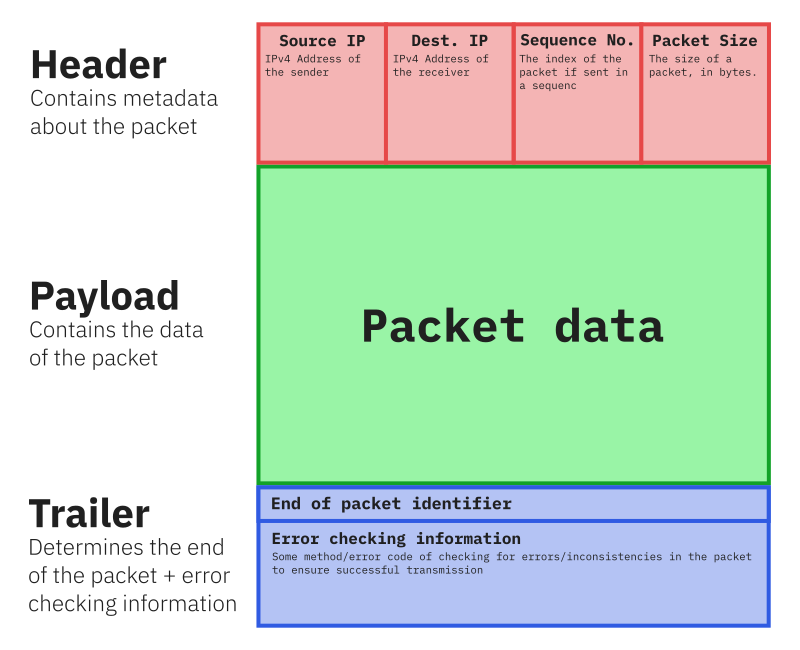
\includegraphics[width=0.6\textwidth]{packet.png}
    \caption{The components of a data packet.}
    \label{fig:packet}
\end{figure}

\subsection{Components of a packet}

Here are they:

\begin{itemize}

\item The Header:
    \begin{itemize}
    \item The IP\footnote{IP Address; in this context, always IPv4 unless if specified} of the sender
    \item The IP of the receiver
    \item The sequence number; If a lot of data must be sent throughout multiple packets, the
          \emph{sequence number} makes sure that the packets' payloads are reassembled in the correct order.
    \item The packet size, in order to make sure the packet received is of the correct size.
    \end{itemize}

\item The payload, which consists of the binary data to be transmitted via the buffer.

\item The trailer, which consists of:
    \begin{itemize}
    \item Some way of identifying the end of the packet. This is typically some special value like a null terminator\footnote{In programming,
          this is referred to as a \emph{sentinel value}, which just means a value that carries some special meaning. An example is like in the
          C programming language, to tell the end of a string, a sentinel value of 0 is used to denote the string finished.}. The algorithm can
          then scan the data until it hit that character to extract the payload.
    \item An error checking method. CRCs are used to check this.
    \end{itemize}
\end{itemize}

\subsection{Packet Switching}

Packet switching is the next step after slicing up data into packets. This is done because sending data across large distances all at once is prone to failure (what happens if a slight portion of the data is corrupted? the data must be sent all over again, taking time). 

This technique involves sending packets onto multiple paths that reach the same destination.

\begin{enumerate}
    \item They begin by being sent out onto the network, from a router.
    \item They each travel separately, but at the same time.
    \item The role of each router/node is to determine which is the most optimal next router to send the packet. For more info on routers, see section \ref{3:sec:routers}. 
    \item When they reach the destination router, as seen in the packet, they are put back together in \emph{sequence number order.}
\end{enumerate}

\begin{figure}[h]
    \centering
    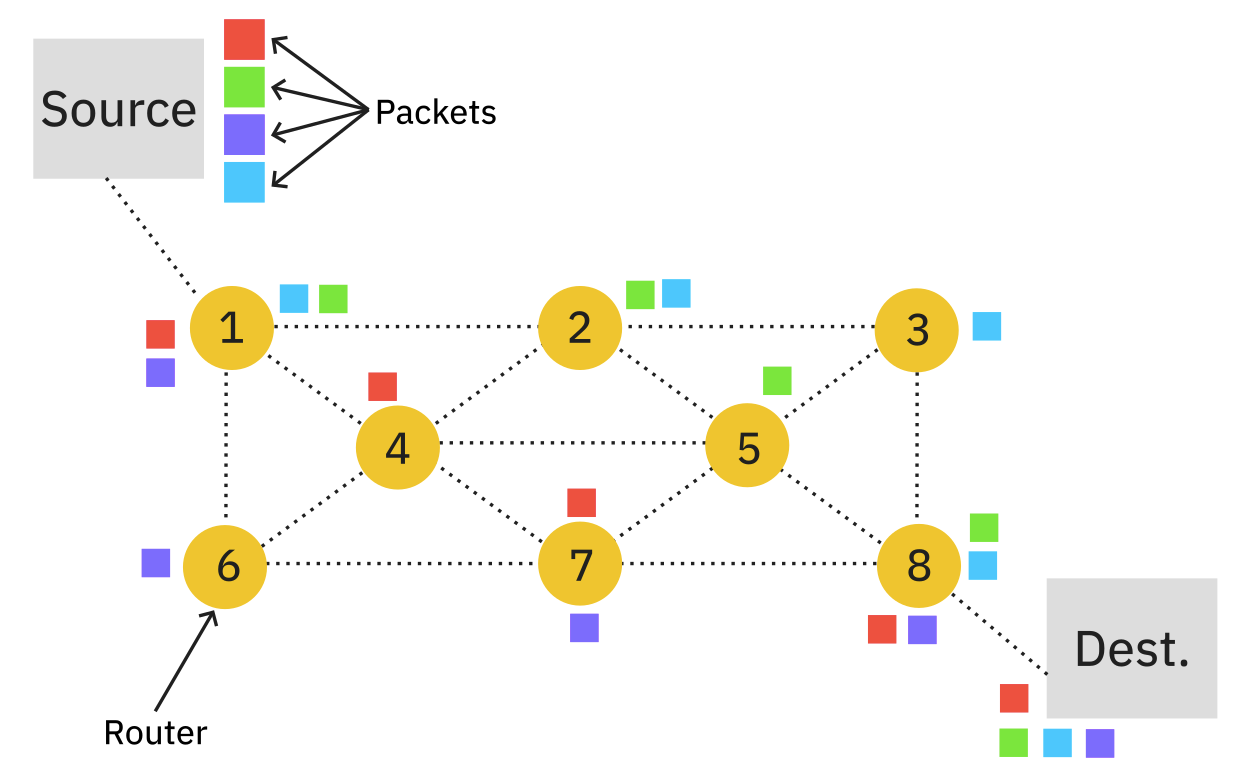
\includegraphics[width=0.7\textwidth]{packetswitching.png}
    \caption{A diagram to illustrate packet switching.}
    \label{fig:packetswitching}
\end{figure}

Each yellow circle can be interpreted as an intersection on a road. The general term for these are nodes, but they are technically just routers.

Figure \ref{fig:packetswitching} has 4 packets that must be sent. The key points are:

\begin{itemize}
    \item The path between the source and the destination are made up of the yellow circles; the nodes.
    \item Each packet takes a different path, i.e. the red packet takes 1-4-7-8, but the blue packet takes 1-2-3-8, etc.
    \item The router at each node will decide the next router the packet should go to. The shortest \emph{available} route is always taken but not the \emph{absolute shortest} route.
    \item When the packets arrive, they will be put back in order according to the sequence number (not depicted).
\end{itemize}

\end{document}
